\documentclass[a4paper,twoside,11pt]{article}

\usepackage{pdfpages}
\usepackage{color}
\definecolor{darkblue}{rgb}{0, 0, 0.5}
\definecolor{listingbg}{gray}{0.95}
\graphicspath{{./figures/}}

\usepackage{amsmath}

\usepackage{xcolor}
\usepackage[most]{tcolorbox}
\usepackage{listings}
\lstloadlanguages{csh, python}
\tcbuselibrary{listings}
\definecolor{light-gray}{gray}{0.95}
% the space reserved between for the ``In'' numbers and the code
\newlength\inwd
\setlength\inwd{1.3cm}
\definecolor{myin}{rgb}{0.039,0.270,1}
\definecolor{myout}{rgb}{0.84,0,0}
\definecolor{mygreen}{rgb}{0,0.4,0}
\definecolor{mykey}{rgb}{0.117,0.403,0.713}
\newcounter{ipythcntr}
\newtcblisting{pyin}[1][]{%
  sharp corners,
  enlarge left by=\inwd,
  width=\linewidth-\inwd,
  enhanced,
  boxrule=0pt,
  colback=light-gray,
  listing only,
  top=0pt,
  bottom=0pt,
  overlay={
    \node[
      anchor=north east,
      text width=\inwd,
      font=\footnotesize\ttfamily\color{myin},
      inner ysep=2mm,
      inner xsep=0pt,
      outer sep=0pt
      ]
      at (frame.north west)
      %{\refstepcounter{ipythcntr}\label{#1}In \theipythcntr:};
      {\refstepcounter{ipythcntr}In \theipythcntr:};
  }
  listing engine=listing,
  listing options={
    aboveskip=1pt,
    belowskip=1pt,
    basicstyle=\small\ttfamily,
    language=Python,
    keywordstyle=\color{mykey},
    showstringspaces=false,
    stringstyle=\color{mygreen}
  },
}
\newtcblisting{pyprint}{
  sharp corners,
  enlarge left by=\inwd,
  width=\linewidth-\inwd,
  enhanced,
  boxrule=0pt,
  colback=white,
  listing only,
  top=0pt,
  bottom=0pt,
  overlay={
    \node[
      anchor=north east,
      text width=\inwd,
      font=\footnotesize\ttfamily\color{mykey},
      inner ysep=2mm,
      inner xsep=0pt,
      outer sep=0pt
      ]
      at (frame.north west)
      {};
  }
  listing engine=listing,
  listing options={
      aboveskip=1pt,
      belowskip=1pt,
      basicstyle=\footnotesize\ttfamily,
      frame=single,
%      language=Python,
      keywordstyle=\color{mykey},
      showstringspaces=false,
      stringstyle=\color{mygreen}
    },
}
\newtcblisting{pyout}[1][\theipythcntr]{
  sharp corners,
  enlarge left by=\inwd,
  width=\linewidth-\inwd,
  enhanced,
  boxrule=0pt,
  colback=white,
  listing only,
  top=0pt,
  bottom=0pt,
  overlay={
    \node[
      anchor=north east,
      text width=\inwd,
      font=\small\ttfamily\color{myout},
      inner ysep=2mm,
      inner xsep=0pt,
      outer sep=0pt
      ]
      at (frame.north west)
      {\setcounter{ipythcntr}{\value{ipythcntr}}Out#1:};
  }
  listing engine=listing,
  listing options={
      aboveskip=1pt,
      belowskip=1pt,
      basicstyle=\small\ttfamily,
      language=Python,
      keywordstyle=\color{mykey},
      showstringspaces=false,
      stringstyle=\color{mygreen}
    },
}


%%\newtcblisting{ipythonnb}[1][\theipythcntr]{
%%  enlarge left by=\inwd,
%%  width=\linewidth-\inwd,
%%  enhanced,
%%  boxrule=0.4pt,
%%  colback=light-gray,
%%  listing only,
%%  top=0pt,
%%  bottom=0pt,
%%  overlay={
%%    \node[
%%    anchor=north east,
%%    text width=\inwd,
%%    font=\footnotesize\ttfamily\color{blue!50!black},
%%    inner ysep=2mm,
%%    inner xsep=0pt,
%%    outer sep=0pt
%%    ]
%%    at (frame.north west)
%%    {\stepcounter{ipythcntr}In [#1]:};
%%  }
%%  listing options={
%%    language=python,
%%    basicstyle=\ttfamily,
%%    escapechar=¢,
%%    showstringspaces=false,
%%  },
%%}

\usepackage{url}
\usepackage{upgreek}
\newcommand{\micron}{\upmu\mathrm{m}}
\usepackage{mathsym}

%%
%% Layout definitions
%%

\usepackage[english]{babel}
\usepackage{lastpage}
\usepackage{multirow}
\usepackage{longtable}
\usepackage{supertabular}
\usepackage{fancyhdr}
\usepackage{graphicx}
\usepackage{mathptmx}
\usepackage{amsmath}
%\usepackage{mathtime}
%\usepackage{verbatim}
%\usepackage[draft]{dmd-doc}
\usepackage{dmd-doc}

\renewcommand{\encodingdefault}{T1}

%%% Local Variables: 
%%% mode: latex
%%% TeX-master: t
%%% End: 

\usepackage[%
   font=small,
   format=plain,
   indention=1.5em,
   labelfont={small,bf},
   up,
   justification=justified,
   singlelinecheck=true]{caption}

\usepackage[%
   pagebackref=true,
   pdfpagelabels=true,
   plainpages=false,
   colorlinks=true]{hyperref}


\dmdTitle{SpecCADO:\\User Manual}
\dmdDocId{}
\dmdIssue{0.1.3}
\dmdDate{19 February 2019}
\dmdPreparedBy{O.\ Czoske}
\dmdPreparedOn{2019-02-19}
\dmdPreparedSig{}
\dmdApprovedBy{}
\dmdApprovedOn{}
\dmdApprovedSig{}
\dmdReleasedBy{}
\dmdReleasedOn{}
\dmdReleasedSig{}

\bibliographystyle{spiebib}   %>>>> makes bibtex use spiebib.bst

\setlongtables

\renewcommand{\topfraction}{1.0}
\renewcommand{\bottomfraction}{1.0}

\newcommand{\brgamma}{\ion{Br}{$\gamma$}~}
\newcommand{\sig}{$\sigma$~}
\newcommand{\m}{$^\mathrm{m}$~}

\newcommand{\aap}{Astronomy \& Astrophysics}
\newcommand{\aaps}{Astronomy \& Astrophysics, Supplement}
\newcommand{\mnras}{Monthly Notices of the Royal Astronomical Society}
\newcommand{\procspie}{Proceedings of the International Society for Optical Engineering}
\newcommand{\pasp}{Publications of the Astronomical Society of the Pacific}
\newcommand{\apjs}{The Astrophysical Journal, Supplement}

\newcommand{\TODO}[1]{\textcolor{red}{\bfseries TODO: #1}}

%%%%%%%%%%%%%%%% BEGIN DOCUMENT %%%%%%%%%%%%%%%%%%%
\begin{document}

% listings style
\lstdefinestyle{csh}{
  basicstyle=\ttfamily,
  columns=flexible,
  frame=single,
  backgroundcolor=\color{listingbg},
  captionpos=b,
  showspaces=false}
\lstset{basicstyle=\ttfamily}
\dmdmaketitle

%\emptypage{This page was intentionally left blank}

\begin{center}
  \textbf{Change record}

  \tablehead{\hline
    \multicolumn{1}{|c|}{Issue/Rev.} &
    \multicolumn{1}{|c|}{Date} &
    \multicolumn{1}{|c|}{Section/Parag.\ affected} &
    \multicolumn{1}{|c|}{Reason/Initiation/Documents/Remarks} \\
    \hline}
  \tabletail{\hline}

  \begin{supertabular}{|l|l|l|l|}
   0.1.3 & 16/2/2019 & All & Layout initialised \\
   \hline
  \end{supertabular}

\end{center}

%\emptypage{This page was intentionally left blank}

\setcounter{tocdepth}{2}
\tableofcontents
\cleardoublepage

%%%%%%%%%%%%%%%%%%%%%%%%%%%%%%%%%%%%%%%%%%%%%%%%%%%%%%%

\section{Scope}
\label{sec:scope}

This document is a brief manual to get users started with SpecCADO,
the spectroscopic simulator for MICADO. SpecCADO is a temporary
package, intended to be merged into SimCADO, the general instrument
data simulator for MICADO in the near future.

SpecCADO depends on SimCADO. For an in-depth description of SimCADO,
we refer to the PDR documentation \cite{SimCADO-PDR}.

\section{Installation}
\label{sec:installation}

The SpecCADO source package can be downloaded from
\url{http://homepage.univie.ac.at/oliver.czoske/speccado-0.1.3.tar.gz}. Unpack
the tar file and change to the source directory:
\begin{lstlisting}[style=csh]
tar xvf speccado-0.1.3.tar.gz
cd speccado-0.1.3/
\end{lstlisting}
It is also possible to obtain SpecCADO from the github repository at
\url{https://github.com/oczoske/SpecCADO}. Note that the latest
snapshots from the repository may not always be perfectly functional.

Install the package by doing
\begin{lstlisting}[style=csh]
pip install .
\end{lstlisting}
or
\begin{lstlisting}[style=csh]
pip install --user .
\end{lstlisting}
The first version may require root permissions; use the second form to
install into a user directory.

If the \lstinline{pip} and \lstinline{python} commands point to a
python-2.7 installation, please try the commands \lstinline{pip3} and
\lstinline{python3} instead.

To test the installation, start a \lstinline{python} or
\lstinline{ipython} session and do
\begin{pyin}
  import speccado
\end{pyin}

\begin{pyin}
speccado.__version__
\end{pyin}
\begin{pyout}
'0.1.3'
\end{pyout}
\begin{pyin}
speccado.bug_report()
\end{pyin}
\begin{pyprint}
Python:
 3.6.0 (default, Feb  6 2017, 15:51:19)
[GCC 4.9.2]

speccado :  0.1.3
simcado :  0.5dev1
astropy :  3.0.5
synphot :  0.1.2
numpy :  1.15.4
scipy :  1.1.0
poppy :  0.7.0
wget :  3.2

Operating system:  Linux
         Release:  4.9.0-0.bpo.8-amd64
         Version:  #1 SMP Debian 4.9.110-3+deb9u5~deb8u1 (2018-10-03)
         Machine:  x86_64
\end{pyprint}

The last command checks that the dependencies are fulfilled. Please
include the output of this command whenever you report a problem or a
possible bug.

The necessary dependencies to run \lstinline{speccado} are
\lstinline{simcado}, \lstinline{astropy}, \lstinline{numpy}, and
\lstinline{scipy}. \lstinline{poppy} and \lstinline{wget} are not
required.

If you want to simulate detector read-out noise, you require the file
\lstinline{FPA_noise.fits}. You can obtain a prepared file by doing
\begin{pyin}
import simcado as sim
sim.get_extras()
\end{pyin}
Unfortunately, this will download a lot of other stuff as well.

\section{Example scripts}
\label{sec:examples}

The subdirectory \lstinline{example/} in the SpecCADO source
distribution includes two example scripts that demonstrate how
SpecCADO works:
\begin{itemize}
\item \lstinline{simulate_example.py} -- simulates spectral traces on
  the MICADO detectors. The slit contains two stars, both of which
  have the same spectrum, viz.~that of GW~Ori, dimmed by 9~magnitudes
  to put it into the usual target range of MICADO.\footnote{No claim
    of scientific realism is made for this example\dots} Atmospheric
  emission is included as a background spectrum that fills the entire
  slit. The spectrum provided in \lstinline{atmo_emission.fits} was
  computed by
  \lstinline{skycalc}.\footnote{\url{https://www.eso.org/observing/etc/skycalc/}}
\item \lstinline{rectify_example.py} -- takes a simulated detector
  frame as input and recifies it into two-dimensional $\xi-\lambda$
  images ($\xi$ is the coordinate along the slit) from which
  one-dimensional spectra can be extracted in the usual way
  (e.g.~using \lstinline{apextract} in Iraf). Note that this is a
  perfect rectification that reverses the transformation applied by
  \lstinline{simulate_example.py}. It does not include the
  uncertainties associated to tracing the spectra in a proper data
  reduction recipe.
\end{itemize}

The \lstinline{example/} directory includes three configuration files
set up for MICADO spectroscopy using the IzJ, J and HK order sorting
filters, respectively. If you run your own simulations, start from one
of these configuration files and modify it according to your needs.

The first parameter in the files is \lstinline{SIM_DATA_DIR}. This is
the directory where SimCADO and SpecCADO look for data files and needs
to be set to where this directory is located on your
system. Typically, this will be the data directory in the SimCADO
source directory, as in
\begin{lstlisting}[style=csh]
SIM_DATA_DIR        /path/to/simcado-0.5dev1/data
\end{lstlisting}
When running the example scripts, the data directory can optionally
also be specified on the command line.

To simulate an HK spectrum of the sources as described above, type the
following at the shell prompt:
\begin{lstlisting}[style=csh]
python simulate_example.py spectro_HK.config <SIM_DATA_DIR>
\end{lstlisting}
It may take about 20~minutes to simulate the nine detectors of the
MICADO focal-plane array. SpecCADO writes a stream of diagnostics to
the screen -- if all goes well this should not be of interest to
anyone except the developer.

The output file is a multi-extension FITS file (one extension per
detector), named \lstinline{detector-<dateTtime>.fits} with
the time stamp of the end of the simulation, for example
\begin{lstlisting}[style=csh]
detector-2019-02-14T17-57-20.fits
\end{lstlisting}

To rectify the spectra run
\begin{lstlisting}[style=csh]
python rectify_example.py detector-2019-02-14T17-57-20.fits
\end{lstlisting}
This currently creates a separate FITS file for each order that is
defined over the entire MICADO wavelength range. Due to the order
sorting filter employed in the simulation, this means that most of the
output files will not contain any signal. The file names are
\lstinline{ORDER-xx_yy.fits} with the numbers identifying the orders
and cross-orders. \textcolor{red}{The output of
  \lstinline{rectify_example.py}
  will be improved.}


\section{Simulation of 2D spectra}
\label{sec:simulation}

In this section, the simulation of detector images will be described
in more detail. This should enable the user to specify sources of
their own.

Any simulation with SpecCADO or SimCADO starts by loading the
configuration file:
\begin{pyin}
import speccado as sc
import simcado as sim

sim_data_dir = "/path/to/simcado-0.5dev1/data/"
cmds = sim.UserCommands("spectro_HK.config", sim_data_dir)
\end{pyin}
The parameter \lstinline{sim_data_dir} can be ignored if
\lstinline{SIM_DATA_DIR} is set correctly within the configuration
file.

It is possible to set individual parameters separately, such as the
exposure time:
\begin{pyin}
cmds['OBS_EXPTIME'] = 60
\end{pyin}
For the simulation of science cases, it is often helpful to turn off
detector saturation:
\begin{pyin}
cmds['FPA_LINEARITY_CURVE'] = 'none'
\end{pyin}
as this makes it possible to simulate long effective exposure times
without the need to break the integration up into several
sub-exposures to avoid saturation.

Currently, SpecCADO only simulates point sources (represented by the
PSF) and background sources (that fill the slit homogeneously).

For point sources, two lists need to be defined, one giving the files
holding the 1D spectra and one giving the positions of the sources in
the slit. The following example assumes two stars are positioned on
the centre line of the slit, both have the same spectrum:
\begin{pyin}
specfiles = ['GW_Ori+9mag.fits', 'GW_Ori+9mag.fits']
sourcepos = [[-1, 0], [1, 0]]
\end{pyin}
The stars are positioned 1~arcsec on either side of the centre of the
3~arcsec slit ($\xi=\pm 1$, $\eta=0$, as defined in
Sect.~\ref{ssec:cube_coordinates}).

Another list gives the background spectra. Here, only one spectrum for
atmospheric emission is provided:
\begin{pyin}
bgfiles = ['atmo_emission.fits']
\end{pyin}

From these lists, a \lstinline{SpectralSource} object is created by
\begin{pyin}
srcobj = sc.SpectralSource(cmds, specfiles, sourcepos, bgfiles)
\end{pyin}

The simulation further requires objects for the PSF and the detector
array:
\begin{pyin}
psfobj = sc.prepare_psf(cmds['SCOPE_PSF_FILE'])
detector = sim.Detector(cmds, small_fov=False)
\end{pyin}
For the detector, we use the \lstinline{Detector} class from
SimCADO. The PSF is a slightly extended form of the SimCADO
\lstinline{PSF} class, created through a SpecCADO function.

The transmission of the optical system (telescope plus instrument) is
extracted from SimCADO's \lstinline{OpticalTrain} class and stored as
an interpolation object that can be evaluated at any wavelength
required for the simulation:
\begin{pyin}
opttrain = sim.OpticalTrain(cmds)
tc_lam = opttrain.tc_mirror.lam_orig
tc_val = opttrain.tc_mirror.val_orig

from scipy.interpolate import interp1d
transmission = interp1d(tc_lam, tc_val, kind='linear',
                        bounds_error=False, fill_value=0.)
\end{pyin}

The optical layout of the spectral traces in the detector focal plane
is described in a FITS file that holds a number of table extensions,
each describing one spectral order.\footnote{The most up to date
  description is \lstinline{specorders-180629.fits}, based on data
  provided by Frank Grupp.}. It is loaded by
\begin{pyin}
tracelist = sc.layout.read_spec_order(cmds['SPEC_ORDER_LAYOUT'])
\end{pyin}

The simulation of the full detector array is then run by
\begin{pyin}
sc.do_all_chips(detector, srcobj, psfobj, tracelist, cmds,
                transmission)
\end{pyin}
The result is written to disk as the multi-extension FITS file
\lstinline{detector-YYYY-MM-DDThh-mm-ss.fits}.

It is also possible to simulate just a single detector from the MICADO
array:
\begin{pyin}
sc.do_one_chip(detector.chips[3], srcobj, psfobj, tracelist, cmds,
               transmission)
\end{pyin}
This simulates chip number~4 of the MICADO array (as python arrays are
zero-offset). The output file in this case is called
\lstinline{chip-YYYY-MM-DDThh-mm-ss.fits}.

\section{Input file format}
\label{sec:input_format}

\subsection{Spectra}
\label{ssec:input_spectra}

Input spectra are expected to provided as one-dimensional FITS images
(\lstinline{NAXIS = 1}). For the transformation from pixels to
wavelengths, a WCS is required in a format that can be read by the
\lstinline{astropy.wcs} module; this includes most formats defined by
Greisen et al.\ (2006) \cite{Greisen2006}. To keep things simple,
spectra sampled on a linear wavelength grid
(\lstinline{CTYPE1='WAVE'}) are recommended. However, frequency or
wave number grids, linear or non-linear, should be possible, if the
WCS is constructed correctly.

As an example, the WCS of the file \lstinline{GW_Ori+9mag.fits} used
in Sect.~\ref{sec:simulation} is
\begin{lstlisting}
NAXIS   =                    1 / number of array dimensions
NAXIS1  =                24750
WCSAXES =                    1 / Number of coordinate axes
CRPIX1  =                  1.0 / Pixel coordinate of reference point
CDELT1  =                6E-11 / [m] Coordinate increment at reference point
CUNIT1  = 'm'                  / Units of coordinate increment and value
CTYPE1  = 'WAVE'               / Vacuum wavelength (linear)
CRVAL1  =           9.9402E-07 / [m] Coordinate value at reference point
\end{lstlisting}

The pixel values have to be in physical units and the units have to be
provided explicitely in the \lstinline{BUNIT} keyword. SpecCADO uses
the very flexible \lstinline{astropy.units} module to convert units:

Input spectra for point sources can be given as photon or energy
fluxes; internally, the units are converted to
$\mathrm{photons}/\mathrm{s}/\mathrm{m^{2}}/\micron$.  Permitted
values for \lstinline{BUNIT} include
\begin{itemize}
\item \lstinline{'erg / (Angstrom cm2 s)'}
\item \lstinline{'ph / (um m2 s)'}
\item \lstinline{'1 / (nm cm2 s)'}
\end{itemize}

Input spectra for background sources can be given as photon or energy
flux densities; internally, the units are converted to
$\mathrm{photons}/\mathrm{s}/\mathrm{m^{2}}/\micron/\mathrm{arcsec^{2}}$. Permitted
values for \lstinline{BUNIT} include
\begin{itemize}
\item \lstinline{'ph / (s m2 micron arcsec2)'}
\item \lstinline{'erg / (s cm2 Angstrom arcmin2)'}
\end{itemize}

\subsection{PSFs}
\label{ssec:input_psf}

The PSF used to place point sources on the slit is provided as a FITS
image in a format that can be read by the SimCADO \lstinline{psf}
module.

The FITS header needs to specify the (effective) wavelength at which
the PSF applies in keyword \lstinline{WAVE0} or
\lstinline{WAVELENG}. SimCADO requires the units to be $\micron$.

In addition, the size of the pixels in the PSF image is required. This
can be given by the keyword \lstinline{PIXSCALE} or the WCS keywords
\lstinline{CDELT1} or \lstinline{CD1_1} (for the PSF a WCS with
\lstinline{CTYPEi='LINEAR'} is adequate). The units are arcsec.

%%%%%%%%%%%%%%%%%%%%%%%%%%%%%%%%%%%%%%%%%%%%%%%%%%%%%%%%%%%%%%%%%%%%%%

\section{Coordinate systems}
\label{sec:coordinates}

\subsection{Detector coordinates}

Detector pixels are characterised by coordinates $(c, i, j)$, where
$c$ is the number of the chip in the MICADO focal plane array
($c=1,\dots,9$; see Fig.~\ref{fig:detector_layout}) and $i$ and $j$
are the column and row number of a pixel ($i, j = 1,\dots,4096$).

\begin{figure}[b]
  \centering
  %\subfigure
  \resizebox{0.6\textwidth}{!}{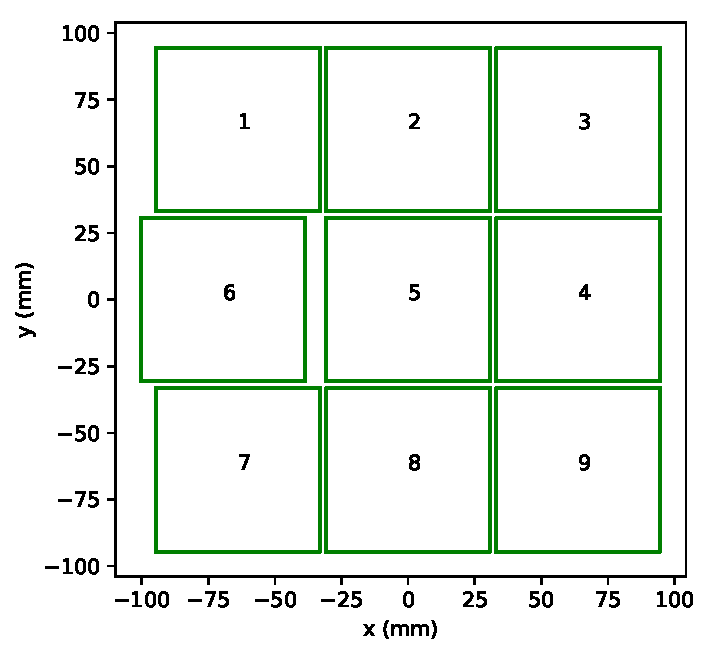
\includegraphics{MICADO_fpa_layout}}
  \caption{Numbering convention of the detectors in the MICADO focal
    plane.}
  \label{fig:detector_layout}
\end{figure}

\subsection{Focal plane coordinates}

A position in the focal plane of MICADO is characterised by the
coordinate pair $(x, y)$, given in millimeters. The origin $x=0$,
$y=0$ is taken to coincide with the centre of detector~5, i.e.~pixel
coordinates $i=2048.5$, $j=2048.5$. The $x$ coordinate increases along
rows of the chips (increasing $i$), the $y$ coordinate increases along
columns of the chips (increasing $j$). Small rotations of the
detectors with respect to the focal plane coordinates are allowed.

The locations of the detector chips within the focal plane are
specified in a focal-plane array definition file that specifies for
each chip the identification number \lstinline{id}; the position of
the chip centre \lstinline{x_cen}, \lstinline{y_cen}; its half width
\lstinline{xhw}, \lstinline{yhw}; the number of pixels in each
direction \lstinline{x_len}, \lstinline{y_len}; the physical pixel
size \lstinline{pixsize}; a rotation angle of the detector rows with
respect to the $x$-axis, \lstinline{angle}; and the detector
\lstinline{gain}.  Listing~\ref{lst:FPA_definition} shows the
focal-plane array definition file for MICADO.

The transformation between pixel coordinates and focal-plane
coordinates is a linear transformation. SimCADO constructs a world
coordinate system (\lstinline{CTYPE}$i$\lstinline{A = 'LINEAR'}) from
the FPA definition file and uses this internally to perform the
transformations. The WCS is written to the SpecCADO output files with
alternative axis descriptor~\lstinline{A} and name
\lstinline{WCSNAMEA = 'PIX2FP'}.


\begin{lstlisting}[style=csh,float, caption=Focal plane array definition file for MICADO with nine HAWAII4RG chips with $15\,\micron$ pixels, label=lst:FPA_definition]
## MICADO H4RG-15 FPA
   id   x_cen  y_cen    xhw    yhw  x_len  y_len  pixsize  angle    gain
#          mm     mm     mm     mm    pix    pix       mm    deg  e-/ADU
    1  -63.84  63.84  30.72  30.72   4096   4096    0.015    0.0     1.0
    2    0.00  63.84  30.72  30.72   4096   4096    0.015    0.0     1.0
    3   63.84  63.84  30.72  30.72   4096   4096    0.015    0.0     1.0
    4  +63.84   0.00  30.72  30.72   4096   4096    0.015    0.0     1.0
    5    0.00   0.00  30.72  30.72   4096   4096    0.015    0.0     1.0
    6  -79.50   0.00  30.72  30.72   4096   4096    0.015    0.0     1.0
    7  -63.84 -63.84  30.72  30.72   4096   4096    0.015    0.0     1.0
    8    0.00 -63.84  30.72  30.72   4096   4096    0.015    0.0     1.0
    9   63.84 -63.84  30.72  30.72   4096   4096    0.015    0.0     1.0
\end{lstlisting}


\subsection{Spectral cube coordinates}
\label{ssec:cube_coordinates}

The spectral source is described as a spectroscopic cube with spatial
coordinates $\xi$ and $\eta$ along and across the slit, respectively
(Fig.~\ref{fig:slit_coords}), and wavelength $\lambda$. Both $\xi$ and
$\eta$ are measured in arcsec, based on the fixed imaging scale of
MICADO. For the short slit of MICADO, $\xi$ runs from
$-1.5\,\mathrm{arcsec}$ to $1.5\,\mathrm{arcsec}$, whereas for the
long slit, $\xi$ runs from $-1.5\,\mathrm{arcsec}$ to
$13.5\,\mathrm{arcsec}$. The slit length to be used can be specified
by the keyword \lstinline{SPEC_SLIT_LENGTH}, the slit width by
\lstinline{SPEC_SLIT_WIDTH}.

\begin{figure}[b]
  \centering
  \resizebox{\textwidth}{!}{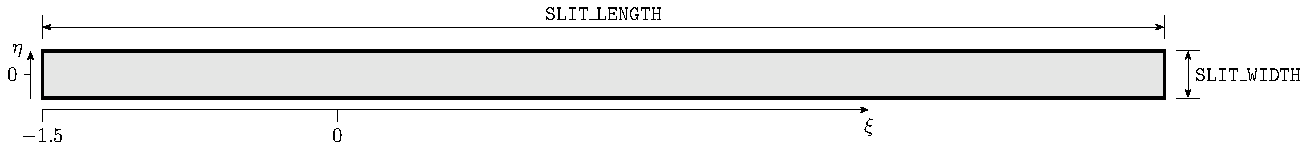
\includegraphics{slit_coords}}
  \caption{Slit coordinates $\xi$, $\eta$ along and across the slit,
    respectively, along with the slit dimensions
    \lstinline{SPEC_SLIT_LENGTH} and \lstinline{SPEC_SLIT_WIDTH}.}
  \label{fig:slit_coords}
\end{figure}

\begin{figure}[b]
  %\subfigure
  \centering
  \resizebox{!}{0.4\textheight}{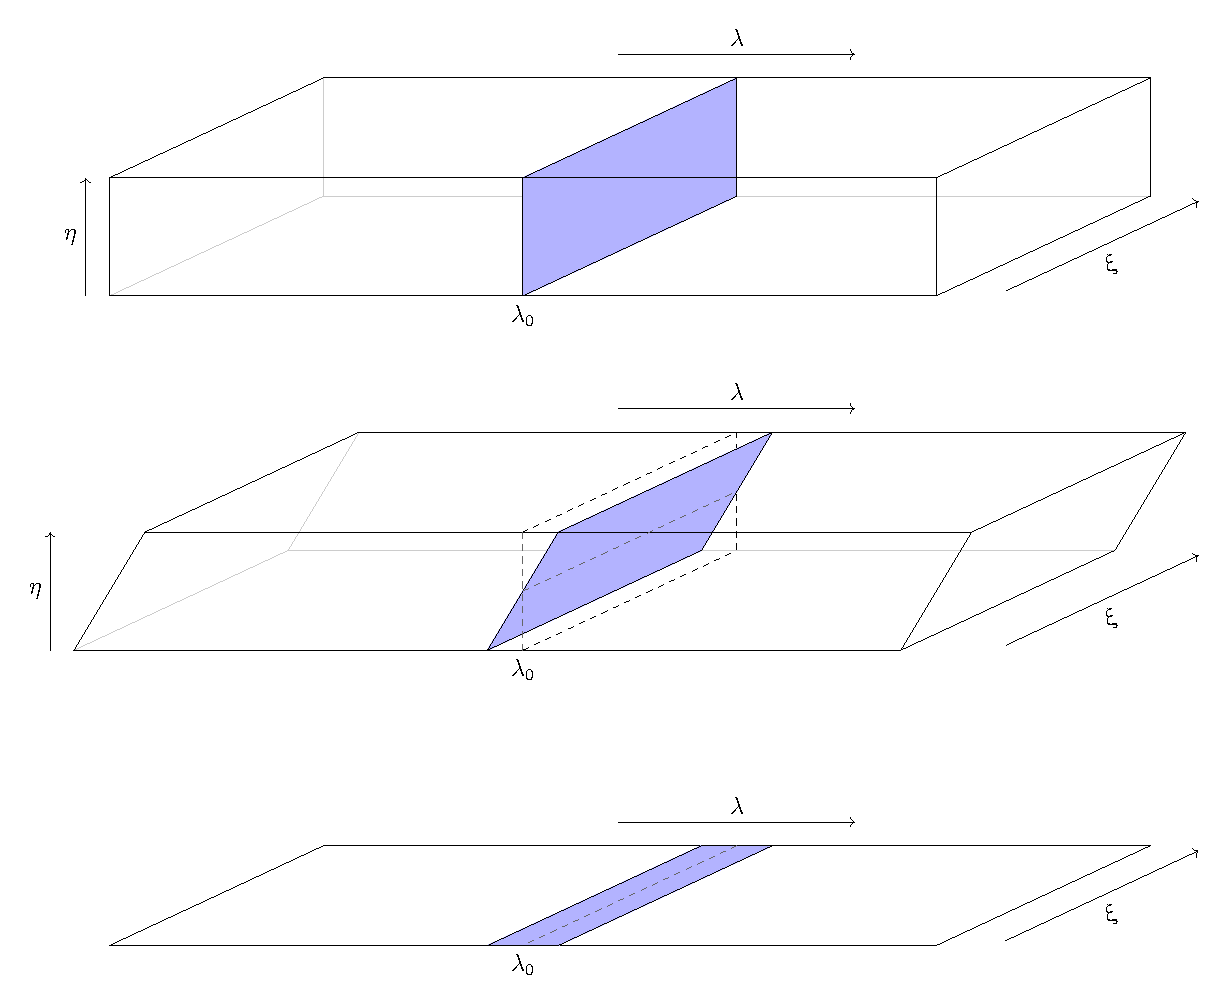
\includegraphics{spectro_cube}}
  \caption{The spectral cube $(\xi, \eta, \lambda)$, top, is sheared
    in the wavelength direction to take into account the slit profile,
    middle, and then summed in the $\eta$ direction to form the
    rectified two-dimensional spectrum $(\xi, \lambda)$, bottom, which
    is subsequently mapped onto the focal plane.}
  \label{fig:cube_collapse}
\end{figure}

The mapping between the centre line of the slit ($\xi$, $\eta=0$,
$\lambda$) and focal-plane coordinates $(x, y)$ for a given spectral
order $s$ is characterised by order-definition files provided by Frank
Grupp. These files were produced using ray-tracing with Zemax and list
matching cube and focal-plane coordinates for a number of
points. SpecCADO models the transformations as fourth-order
polynomials fitted to the order definition files:

\begin{eqnarray}
  x(\xi, \lambda) &=& \sum_{i,j=0}^{4} A_{s,ij}\,\xi^{i}\,\lambda^{j} \label{eq:xilam2x} \\
  y(\xi, \lambda) &=& \sum_{i,j=0}^{4} B_{s,ij}\,\xi^{i}\,\lambda^{j} \label{eq:xilam2y} \\
  \xi(x, y)     &=& \sum_{i,j=0}^{4} C_{s,ij}\,x^{i}\,y^{j} \label{eq:xy2xi} \\
  \lambda(x, y) &=& \sum_{i,j=0}^{4} D_{s,ij}\,x^{i}\,y^{j} \label{eq:xy2lam}
\end{eqnarray}

The across-slit coordinate $\eta$ is integrated out before the
spectral cube is mapped to the focal plane as illustrated in
Fig.~\ref{fig:cube_collapse}. A monochromatic slice
$\lambda=\lambda_{0}$ of the spectral cube is mapped to a rectangle in
the focal plane. Given a unique mapping of focal-plane coordinates to
wavelength (the wavelength calibration) this means that, say, the top
of the slit will be at an offset wavelength,
$\lambda_{0}+\Delta\lambda$. If the slit width (given by the SimCADO
keyword \lstinline{SPEC_SLIT_WIDTH}) is $b$ and the plate scale is $p$
(in $\mathrm{mas}\,\micron^{-1}$), then the wavelength shift is
\begin{equation}
  \Delta\lambda = \frac{\partial\lambda}{\partial y}\,\Delta y
  = \frac{b}{2}\frac{1}{p} \left[\frac{\partial y}{\partial
      \lambda}(\xi, \lambda)\right]^{-1}
\end{equation}

Each plane ($\eta = \mathrm{const.}$) of the spectral cube is shifted
by the appropriate amount in the wavelength direction. The resulting
sheared cube is then summed in the $\eta$ direction to give a
two-dimensional spectrum with the spectral lines automatically
broadened by the slit profile. The transformations (\ref{eq:xilam2x})
and (\ref{eq:xilam2y}) are then applied to map the 2D spectrum into
the focal plane and onto the detectors.


\section{Spectral layout}
\label{sec:spectral_layout}

The panels in Fig.~\ref{fig:spectral_layout} show the spectral traces
for the 3~arcsec slit and the three order sorting filters,
\textit{IzJ}, \textit{J} and
\textit{HK}. Fig.~\ref{fig:spectral_orders_wavelength} identifies the
orders as a function of wavelength.

\begin{figure}[hb]
  \centering
  %\subfigure
  \resizebox{0.47\textwidth}{!}{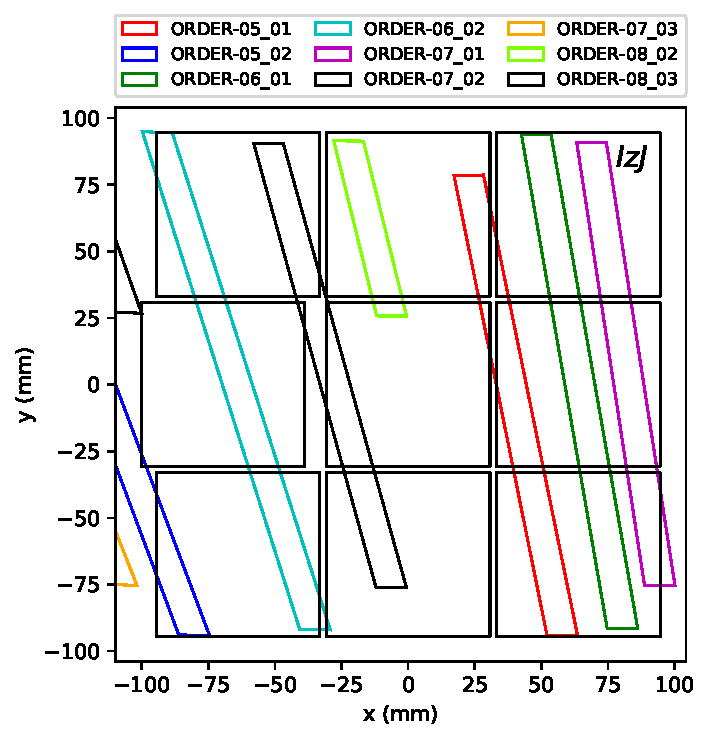
\includegraphics{spectro_IJ_layout}}
  \resizebox{0.47\textwidth}{!}{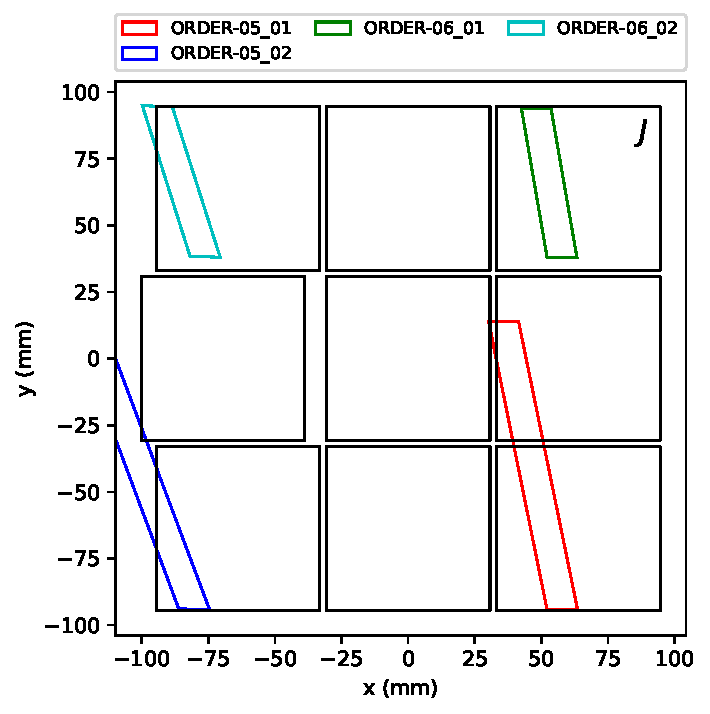
\includegraphics{spectro_J_layout}}\\
  \resizebox{0.47\textwidth}{!}{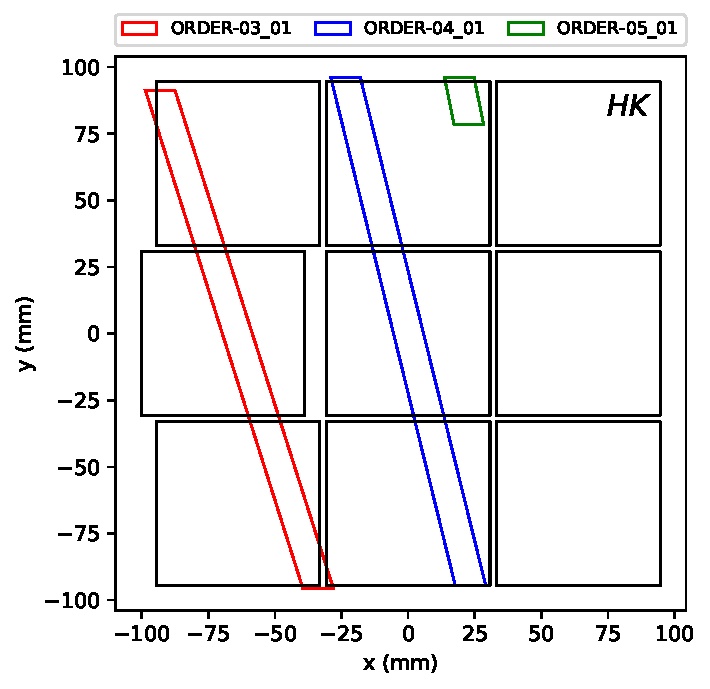
\includegraphics{spectro_HK_layout}}
  \caption{Spectral layout based on the PDR design. The slit has a
    width of 3~arcsec on the sky.}
  \label{fig:spectral_layout}
\end{figure}

\begin{figure}[ht]
  \centering
  \resizebox{\textwidth}{!}{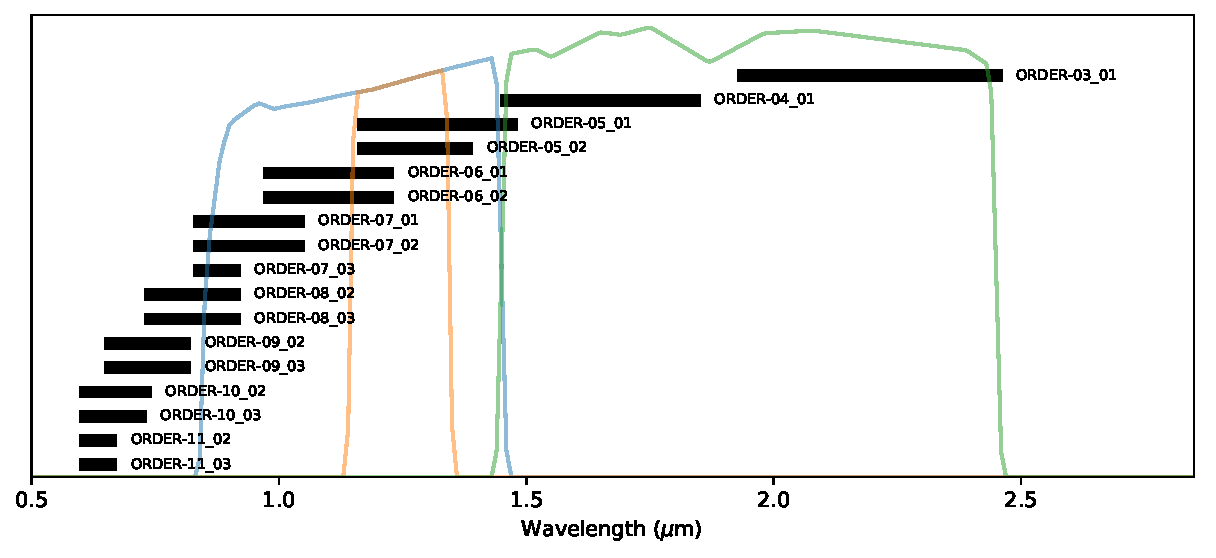
\includegraphics{spectral_orders_v_wavelength}}
  \caption{Wavelength ranges covered by the spectral orders. The blue,
    orange and green curves give the relative system transmissivities
    for the IzJ, J and HK order sorting filters, respectively.}
  \label{fig:spectral_orders_wavelength}
\end{figure}

%%%%%%%%%%%%%%%%%%%%%%%%%%%%%%%%%%%%%%%%%%%%%%%%%%%%%%%%%

\phantomsection
\addcontentsline{toc}{section}{References}
\label{sec:references}
\bibliography{references}   %>>>> bibliography data in report.bib

\end{document}
